\documentclass[10pt]{beamer}

\usepackage[utf8]{inputenc}
\usepackage{pgfpages}
\usepackage{dirtree}
\setbeamertemplate{note page}[plain]
\AtEndNote{\vfill \begin{center} mm:hh \end{center}}
\newcommand{\notedir}[1] {
  \note{\dirtree{#1}}}
\usepackage{tcolorbox}
\usepackage{tikz}
\usepackage{tikz-3dplot}
\usetikzlibrary{intersections,calc,,angles,quotes,through}
\usepackage{amsmath}
\usepackage{graphicx}
\usepackage{cases}
\def \heart {\textcolor{blue}{$\heartsuit$} }
\def \C {\mathcal{C}}
\def \orthog {\underline{\perp}}
\def\arcos{\operatorname{arcos}}
\def \deg {^{\circ}}

\newcommand{\vect}[1] {
  \overrightarrow{#1}}

\tcbset{%
	basic/.style={colframe=black,
		      colback=white,
		      top= 0mm,
		      bottom = 2mm,
		      boxsep=0mm
		      }
}
\tikzset{
    invisible/.style={opacity=0},
    visible on/.style={alt={#1{}{invisible}}},
    alt/.code args={<#1>#2#3}{%
      \alt<#1>{\pgfkeysalso{#2}}{\pgfkeysalso{#3}} % \pgfkeysalso doesn't change the path
    },
  }

    
\begin{document}  
    \beamertemplatenavigationsymbolsempty
    \setlength{\abovedisplayskip}{0pt}
    \setlength{\belowdisplayskip}{0pt}
    \frame{ \frametitle{Perpendicularité.} \underline{Droite $\bot$ plan.}\\ \bigskip
	  \begin{figure}[h]
				  \begin{tikzpicture}[scale=0.85]
			          %projection ($(X)!(B')!(B)$)
			          %nommer chemin 'name path
			          %intersection \path [name intersections={of=d and gb,by=G}];
			          
			          %\draw[help lines] (-3,-3) grid (3,3);
			          \draw[dotted] (2,0,0) -- (2,0,2) node[above left]{$\pi$} -- (-2,0,2) -- (-2,0,0);
			          \coordinate[label=above:$d$](P) at (0,0.8,1);
			          
			         
			          \draw (P) -- (0,0,1);
			          \draw (0,0,1) -- (0,-0.5,1);
			          \draw (0,0,0.85) -- (0,0,1.15) (-0.08,0,1) -- (0.08,0,1);
			          \draw(-1,0,-0.5) -- (-0.5,0,1.8)node[below]{$d_1$};
			          \draw(-0.7,0,-0.5) -- (-0.8,0,1.8)node[below left]{$d_2$};
				  \end{tikzpicture}
				  \end{figure} \bigskip
				  
				  
				   \textit{Condition} : Droite orthogonale à deux droites sécantes du plan. \\ \bigskip
				   \textit{Implication} : Droite orthogonale à toutes les droites du plan.
				  
  \notedir{%
  .1 Perpendicularité droite - plan.
  .2 Condition : droite orthogonale à 2 droites sécantes du plan..
  .2 Implication : droite orthogonale à tt droites du plan..
  }
    }

    \frame{ \frametitle{Positions relatives de deux droites.}
    \begin{columns}[t]
     \column{.3333\textwidth}
				  \begin{figure}[h]
				  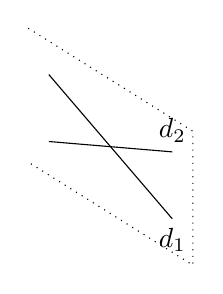
\begin{tikzpicture}[scale=0.85]
			          %projection ($(X)!(B')!(B)$)
			          %nommer chemin 'name path
			          %intersection \path [name intersections={of=d and gb,by=G}];
			          
			          %\draw[help lines] (-3,-3) grid (3,3);
			          \draw[dotted] (-2,2,-2) -- (2,2,2) node[above left]{} -- (2,0,2) -- (-2,0,-2);
			          \draw (-1.5,1.5,-1.5) -- (1.5,0.5,1.5)node[below]{$d_1$};
			          \draw (1.5,1.5,1.5)node[above]{$d_2$} -- (-1.5,0.5,-1.5);
				  \end{tikzpicture}
				  \end{figure}
				  \textit{Sécantes} : coplanaires et non parallèles.
     \column{.34\textwidth}
				  \begin{figure}[h]
				  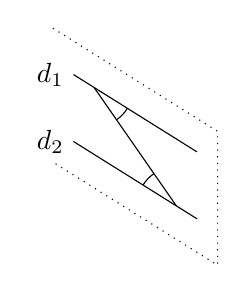
\begin{tikzpicture}[scale=0.85]
			          %projection ($(X)!(B')!(B)$)
			          %nommer chemin 'name path
			          %intersection \path [name intersections={of=d and gb,by=G}];
			          
			          %\draw[help lines] (-3,-3) grid (3,3);
			          \draw[dotted] (-2,2,-2) -- (2,2,2) node[above left]{} -- (2,0,2) -- (-2,0,-2);
			          \draw (-1.5,1.5,-1.5)node[left](d_1){$d_1$} -- (1.5,1.5,1.5);
			          \draw (1.5,0.5,1.5) -- (-1.5,0.5,-1.5)node[left]{$d_2$};
			          \draw (-1,1.5,-1) -- (1,0.5,1);
			          \coordinate (A) at (-1,1.5,-1);
			          \coordinate (B) at (1,0.5,1);
			          \coordinate (C) at (1.5,1.5,1.5);
			          \coordinate (D) at (-1.5,0.5,-1.5);
			          \pic [draw, angle eccentricity=1.5] {angle = B--A--C};
			          \pic [draw, angle eccentricity=1.5] {angle = A--B--D};
				  \end{tikzpicture}
				  \end{figure}
				  \textit{Parallèles} : coplanaires et angles correspondants  égaux.
	\column{.3333\textwidth}
				  \begin{figure}[h]
				  \begin{tikzpicture}[scale=0.85]
			          %projection ($(X)!(B')!(B)$)
			          %nommer chemin 'name path
			          %intersection \path [name intersections={of=d and gb,by=G}];
			          
			          %\draw[help lines] (-3,-3) grid (3,3);
			          
			          \draw (-1.5,1.5,-1.5)node[left](d_1){$d_1$} -- (1.5,1.5,1.5);
			          \draw (1.5,0.5,0) -- (-1.5,0.5,0)node[left]{$d_2$};
				  \end{tikzpicture}
				  \end{figure} \vspace{3.4em}
				  \textit{Gauches} : ni parallèles ni sécantes.			  
    \end{columns}

	\notedir{%
	.1 Positions des droites.
	.2 Sécantes si coplanaires et non parallèles..
	.2 Parallèles si coplanaires et angles correspondants égaux..
	.2 Gauches si ni sécantes ni parallèles..
	} 
    }
	  
  
\end{document}

%%% Local Variables:
%%% mode: latex
%%% TeX-master: t
%%% End:
